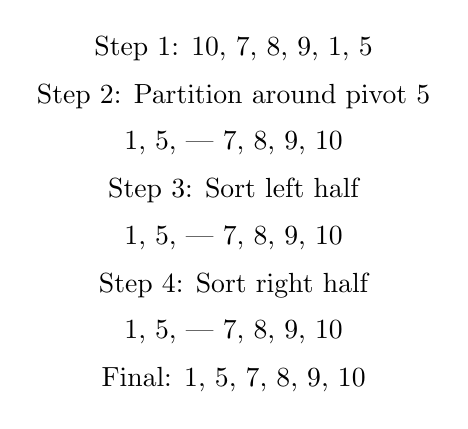
\begin{tikzpicture}[scale=1.2]
    % Initial unsorted array
    \node at (0, 4) {Step 1: 10, 7, 8, 9, 1, 5};

    % Partitioning step: pivot 5
    \node at (0, 3.5) {Step 2: Partition around pivot 5};

    % After first partition
    \node at (0, 3) {1, 5, | 7, 8, 9, 10};

    % Recursively sorting left half
    \node at (0, 2.5) {Step 3: Sort left half};

    % Left half sorted
    \node at (0, 2) {1, 5, | 7, 8, 9, 10};

    % Recursively sorting right half
    \node at (0, 1.5) {Step 4: Sort right half};

    % Right half sorted
    \node at (0, 1) {1, 5, | 7, 8, 9, 10};

    % Final sorted array
    \node at (0, 0.5) {Final: 1, 5, 7, 8, 9, 10};
\end{tikzpicture}
